\documentclass[autodetect-engine,dvipdfmx-if-dvi,ja=standard,a4j,jbase=11pt,magstyle=nomag*]{bxjsreport}
% \documentclass[uplatex, dvipdfmx, a4paper, 11ptj, report]{jsbook}
% small japanese font size:     9pt, 10pt, 11pt, 12pt, 14pt, ... (please refer the document of jsclasses)
% word-like japanese font size: 10ptj 10.5ptj, 11ptj, 12ptj (or jbase=xxpt (without 'j') if error is occured)

\usepackage{ifptex,ifxetex,ifluatex}
\ifluatex
    \usepackage{bxcalcux}
    \ltjsetparameter{jacharrange={-2,-3}}
    \usepackage{luatexja-otf}
    \usepackage{bxbase}
\else\ifxetex
    % \usepackage{zxjatype}
    % \usepackage[macros]{zxotf}
    \XeTeXgenerateactualtext=1
    \usepackage{xltxtra}
    \usepackage{bxbase}
\else\ifuptex
    \usepackage{otf}
    \usepackage[prefernoncjk]{pxcjkcat}
    \cjkcategory{sym11,sym18,sym19}{cjk}
    \usepackage[utf8]{inputenc}
    \usepackage{pxbase}
\else\ifstrictptex
    \usepackage{otf}
    \usepackage[utf8]{inputenc}
    \usepackage{pxbase}
\fi\fi\fi\fi

\usepackage[LGR,T2A,T1]{fontenc}

\usepackage{graphicx}
% \usepackage[dvipdfmx]{graphicx}
\usepackage{grffile}

% paper layout setting
\setpagelayout{noheadfoot, left=18.0truemm, right=18.0truemm, top=29.0truemm, bottom=26.0truemm, columnsep=6.5truemm}
% \setpagelayout{noheadfoot, left=15.0truemm, right=5.0truemm, top=12.5truemm, bottom=12.5truemm, columnsep=5.0truemm}

% font setting
\usepackage{amsmath}
\usepackage{amssymb}
\usepackage{mathtools}
\usepackage{bm}
\usepackage{fix-cm}
\usepackage{newtxtext}
\usepackage[slantedGreek]{newtxmath}

% caption setting
\usepackage[font=bf,labelfont=bf,labelsep=quad]{caption}

% to balance the last page of the two-column article
% \usepackage[nospread, keeplastbox, nodebug]{flushend}

% title font style
\renewcommand{\headfont}{\bfseries}

% section setting (using titlesec, uelm package)
\renewcommand{\thesection}{\arabic{section}}
\renewcommand{\thesubsection}{\arabic{section}.\arabic{subsection}}

\usepackage[explicit]{titlesec}
\usepackage[normalem]{ulem}
\titleformat{name=\section}{\normalfont\headfont\normalsize\raggedright}{}{0pt}{\uline{\thesection.\quad#1}}
\titleformat{name=\section,numberless}{\normalfont\headfont\normalsize\raggedright}{}{0pt}{\uline{#1}}
% \titleformat{name=\section}{\normalfont\headfont\normalsize\raggedright}{}{0pt}{\thesection.\quad#1}
\titlespacing{name=\section}{0pt}{.5\Cvs plus .0\Cvs minus .3\Cvs}{.1\Cvs plus .0\Cvs minus .1\Cvs}
\titleformat{name=\subsection}{\normalfont\headfont\normalsize\raggedright}{}{0pt}{\thesubsection.\quad#1}
\titleformat{name=\subsection,numberless}{\normalfont\headfont\normalsize\raggedright}{}{0pt}{#1}
\titlespacing{name=\subsection}{0pt}{.3\Cvs plus .0\Cvs minus .2\Cvs}{.0\Cvs plus .0\Cvs minus .0\Cvs}

% \makeatletter
% \renewcommand{\section}{\@startsection{section}{1}{\z@}{.5\baselineskip}{.1\baselineskip}{\normalfont\normalsize\headfont\raggedright}}
% \renewcommand{\subsection}{\@startsection{subsection}{2}{\z@}{.3\baselineskip}{\z@}{\normalfont\normalsize\headfont\raggedright}}
% \makeatother

\usepackage{secdot}
\sectiondot{section}
\sectiondot{subsection}

% list (itemize, enumerate, description, ...)
\usepackage{enumitem}
\setlist[1]{parsep=.0\baselineskip,topsep=.2\baselineskip,itemsep=.1\baselineskip}
% \makeatletter
% \def\@listi{\leftmargin\leftmargini
%     \parsep \z@
%     \topsep .2\baselineskip
%     \itemsep .1\baselineskip \relax}
% \let\@listI\@listi
% \makeatother

% no page number
\pagestyle{empty}

% footnote
\usepackage[bottom,hang,stable]{footmisc}
\setlength{\footnotemargin}{0pt}

% float setting (figure, table)
\setlength\floatsep{2.0truemm}
\setlength\textfloatsep{2.0truemm}
\setlength\intextsep{1.0truemm}
\setlength\dblfloatsep{2.0truemm}
\setlength\dbltextfloatsep{2.0truemm}
\setlength\abovecaptionskip{0.5truemm}
\setlength\belowcaptionskip{0.5truemm}

% lineskip setting (body text, display-style equation)
\AtBeginDocument{%
    \narrowbaselines    % basic english lineskip (for article)
    % \widebaselines      % basic japanese lineskip
    %
    \setlength\abovedisplayskip{1.5truemm}    % equation setting
    \setlength\belowdisplayskip{1.5truemm}    % equation setting
}

% to suit ms-word template
\renewcommand{\baselinestretch}{0.9}


\makeatletter
%
% maketitle
% additional elements
\newcommand*{\etitle}[1]{\gdef\@etitle{#1}}
\newcommand*{\studentid}[1]{\gdef\@studentid{#1}}
\newcommand*{\laboarea}[1]{\gdef\@laboarea{#1}}
\newcommand*{\laboname}[1]{\gdef\@laboname{#1}}
%
% style definition
\def\@maketitle{%
\newpage%
\centering%
\let\footnote\thanks%
%
% title
{\fontsize{16.00truept}{16.00truept}\selectfont\headfont\@title\par}%
%
% english title
\ifx\@etitle\@undefined\else{\vspace{1truemm}{\fontsize{12truept}{12truept}\selectfont\headfont\@etitle\par}}\fi%
%
% name (option: student id)
\vspace{1truemm}%
\ifx\@studentid\@undefined\else{\fontsize{12truept}{12truept}\selectfont\headfont\@studentid\hspace{\Cwd}}\fi%
{\fontsize{12truept}{12truept}\selectfont\headfont\@author\par}%
%
% research area (\laboarea) and laboratory name (\laboname)
\ifx\@laboarea\@undefined%
    \ifx\@laboname\@undefined%
    \else\vspace{1truemm}{\fontsize{12truept}{12truept}\selectfont\headfont\@laboname\par}%
    \fi%
\else%
    \ifx\@laboname\@undefined\vspace{1truemm}{\fontsize{12truept}{12truept}\selectfont\headfont\@laboarea\par}%
    \else\vspace{1truemm}{\fontsize{12truept}{12truept}\selectfont\headfont\@laboarea\hspace{\Cwd}\@laboname\par}%
    \fi%
\fi%
%
%% old version (2 line) of research area (\laboarea) and laboratory name (\laboname)
%\ifx\@laboarea\@undefined\else{\vspace{1truemm}{\fontsize{10truept}{10truept}\selectfont\@laboarea\par}}\fi%
%\ifx\@laboname\@undefined\else{\vspace{1truemm}{\fontsize{10truept}{10truept}\selectfont\@laboname\par}}\fi%
%
%% date (error)
% \ifvoid\@date\else{\vspace{2truemm}{\fontsize{12truept}{12truept}\selectfont\@date\par}}\fi%
%
% abstract (no check)
\ifvoid\@abstractbox\else{\vspace{2truemm}{\centering{\fontsize{10truept}{10truept}\selectfont\box\@abstractbox\par}}}\fi%
\vspace{2truemm}%
}
%
%
% bibliography
\newcommand{\@bibsection}{\@startsection{section}{1}{\z@}{.5\baselineskip}{0.2\baselineskip}{\normalfont\fontsize{9truept}{11truept}\selectfont\headfont\raggedright}}
\setlength\bibindent{\Cwd}
\renewenvironment{thebibliography}[1]{%
    \global\let\presectionname\relax
    \global\let\postsectionname\relax
    \@bibsection*{\refname}\@mkboth{\refname}{\refname}%
    \list{\@biblabel{\@arabic\c@enumiv}}{%
        \settowidth\labelwidth{\@biblabel{#1}}%
        \leftmargin\labelwidth
        \advance\leftmargin\labelsep
        \setlength\itemsep{0.5truept plus 1.0truept minus 0.5truept}
        \@openbib@code
        \usecounter{enumiv}%
        \let\p@enumiv\@empty
        \renewcommand\theenumiv{\@arabic\c@enumiv}}%
    \fontsize{8truept}{9.5truept}\selectfont
    \sloppy
    \clubpenalty4000
    \@clubpenalty\clubpenalty
    \widowpenalty4000%
    \sfcode`\.\@m}
{\def\@noitemerr{\@latex@warning{Empty `thebibliography' environment}}\endlist}
%
\makeatother


\mainmatter
\setchapterxr[thesis][bibliography]{5}


\begin{document}


\chapter[実環境における評価実験]{実環境における評価実験}
\label{chap:sim_nao}


\section{はじめに}
本章では,4章で実装したシステムを用いて実機実験を行うための,実験設定とその結果について説明し
,考察を行う.



\section{実験設定}
実機を実装した実験は2つ行った.1つ目の実験は大阪市立大学の野球場,2つ目の実験は大阪市立大学のハンドボールコートで行った.以下に2つの実験で共通の設定を述べる.\cref{fig:ground}にハンドボールコートと野球場の位置を示す.

東をx軸正方向,北をy軸正方向とし
1[m]を軸の1目盛りとするmap座標系を考える.原点を中心に10[m]を1辺の長さとして正方形の領域を人物の行動可能領域とする.
その領域の東側,西側,北側,南側の辺から10[m]$times$15[m]の長方形の領域をUAVの飛行範囲と設定する.
基準とするLiDARを北向きに設置しその位置をmap座標系の(0.0, -5.0)と定義することで原点の座標とGPS位置を逆算する.
2台目のLiDARは南向きに任意の位置に置くことで原点のGPS座標を用いてmap座標を得ることができる.
\cref{fig:picture}に実機実験を行っている様子を示す.

\begin{figure}[h]
    \centering
    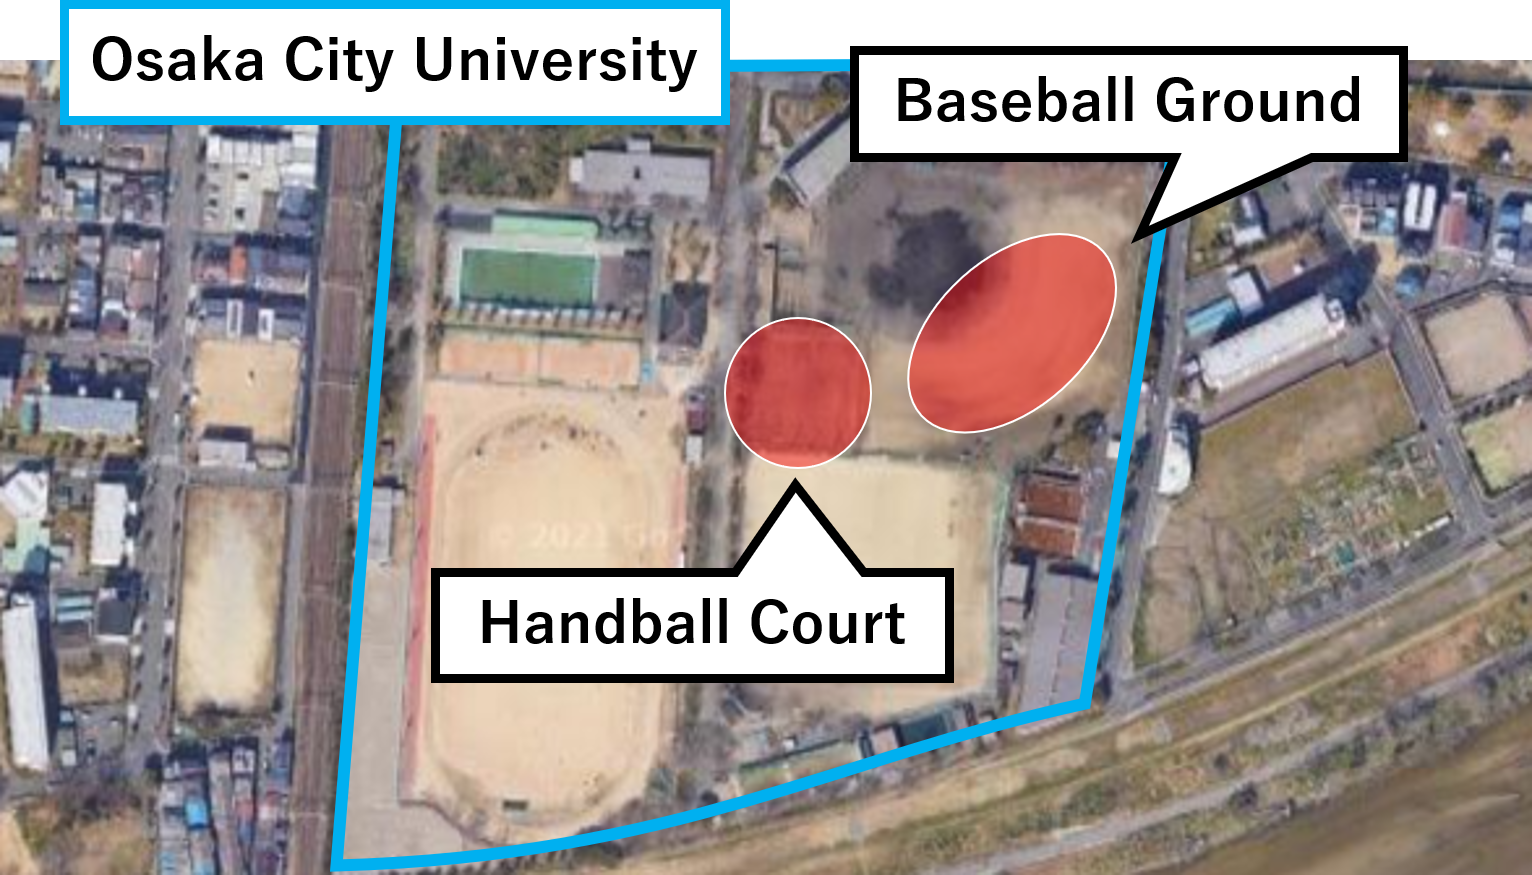
\includegraphics[width=0.8\linewidth, clip]{./figure/chapter5/ground.png}
    \caption{Handball Court and Baseball Ground in Osaka City Univercity}
    \label{fig:ground}
\end{figure}

\begin{figure}[h]
    \centering
    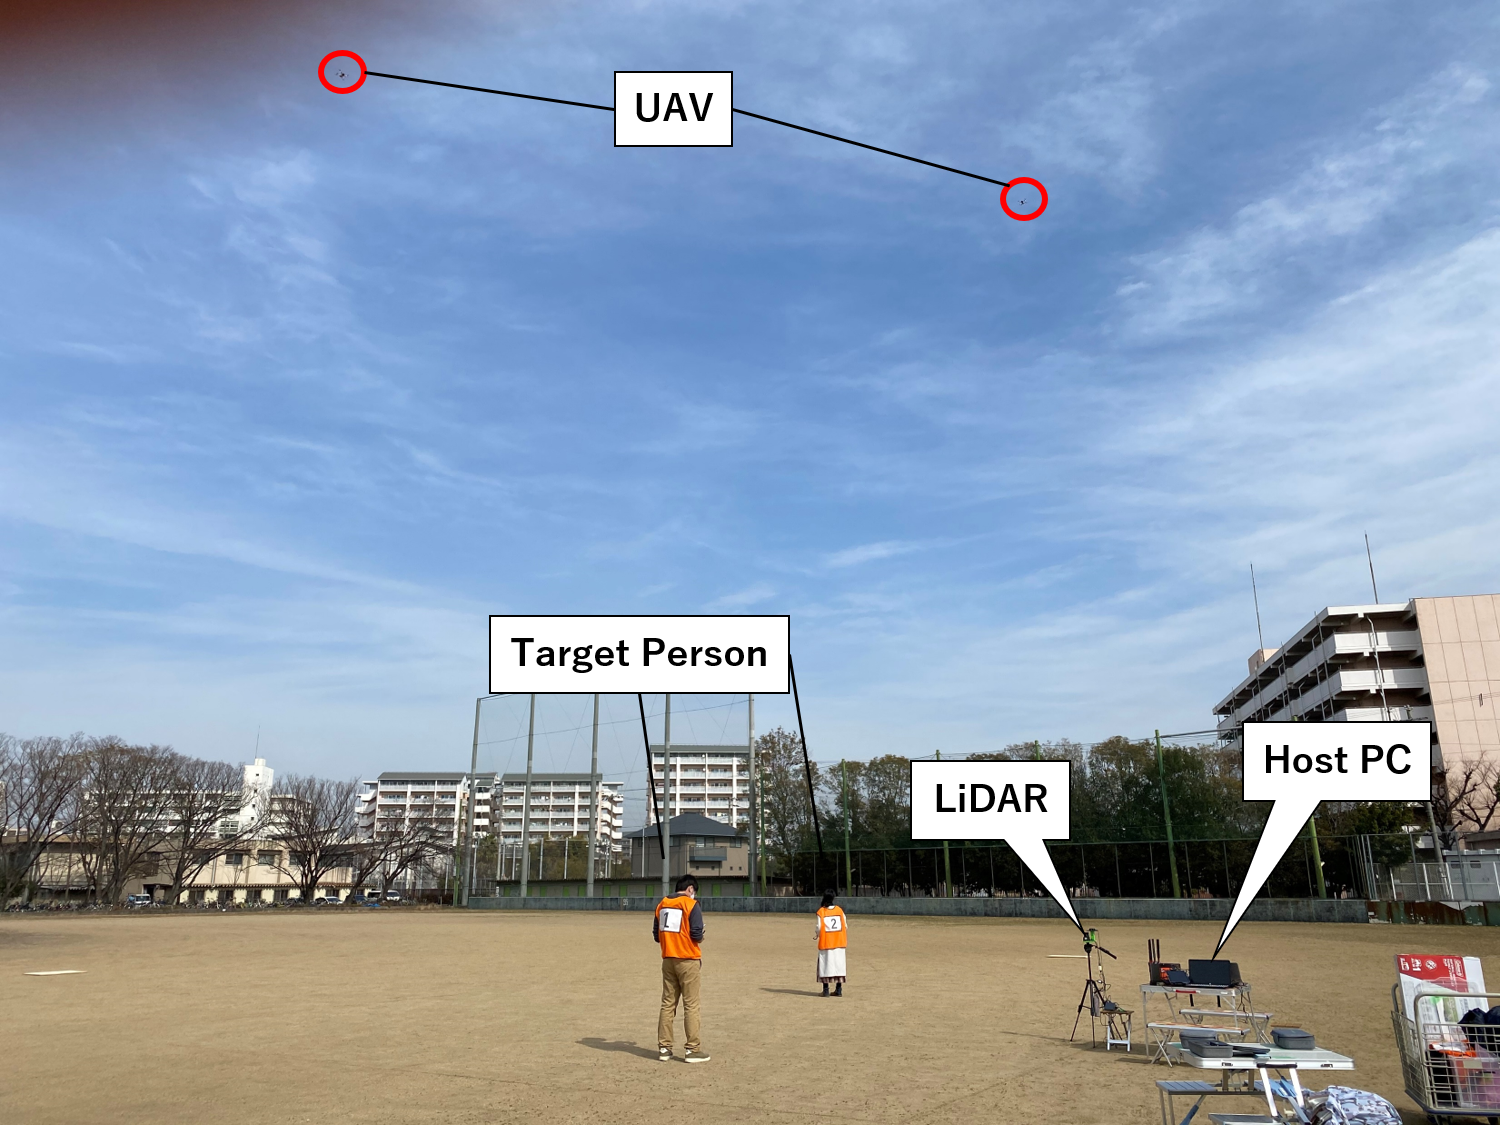
\includegraphics[width=0.8\linewidth, clip]{./figure/chapter5/picture.png}
    \caption{Experimental Scenery}
    \label{fig:picture}
\end{figure}

\newpage
\subsection{ダミーを配置した場合の撮影計画}
1つ目の実験として,1台のLiDARに対して人物行動領域内に複数の人物を配置し,
ダミーを配置する場合とダミーを配置しない場合の双方で撮影計画を行い,
UAVの目標移動位置の比較を行う.
この実験では1台のUAVを北側の飛行可能範囲に配置し,
ダミーを配置した場合と配置しない場合のUAVの目標位置の比較を行う.
\cref{fig:env}にフィールドの設定を示す.

\begin{figure}[h]
    \centering
    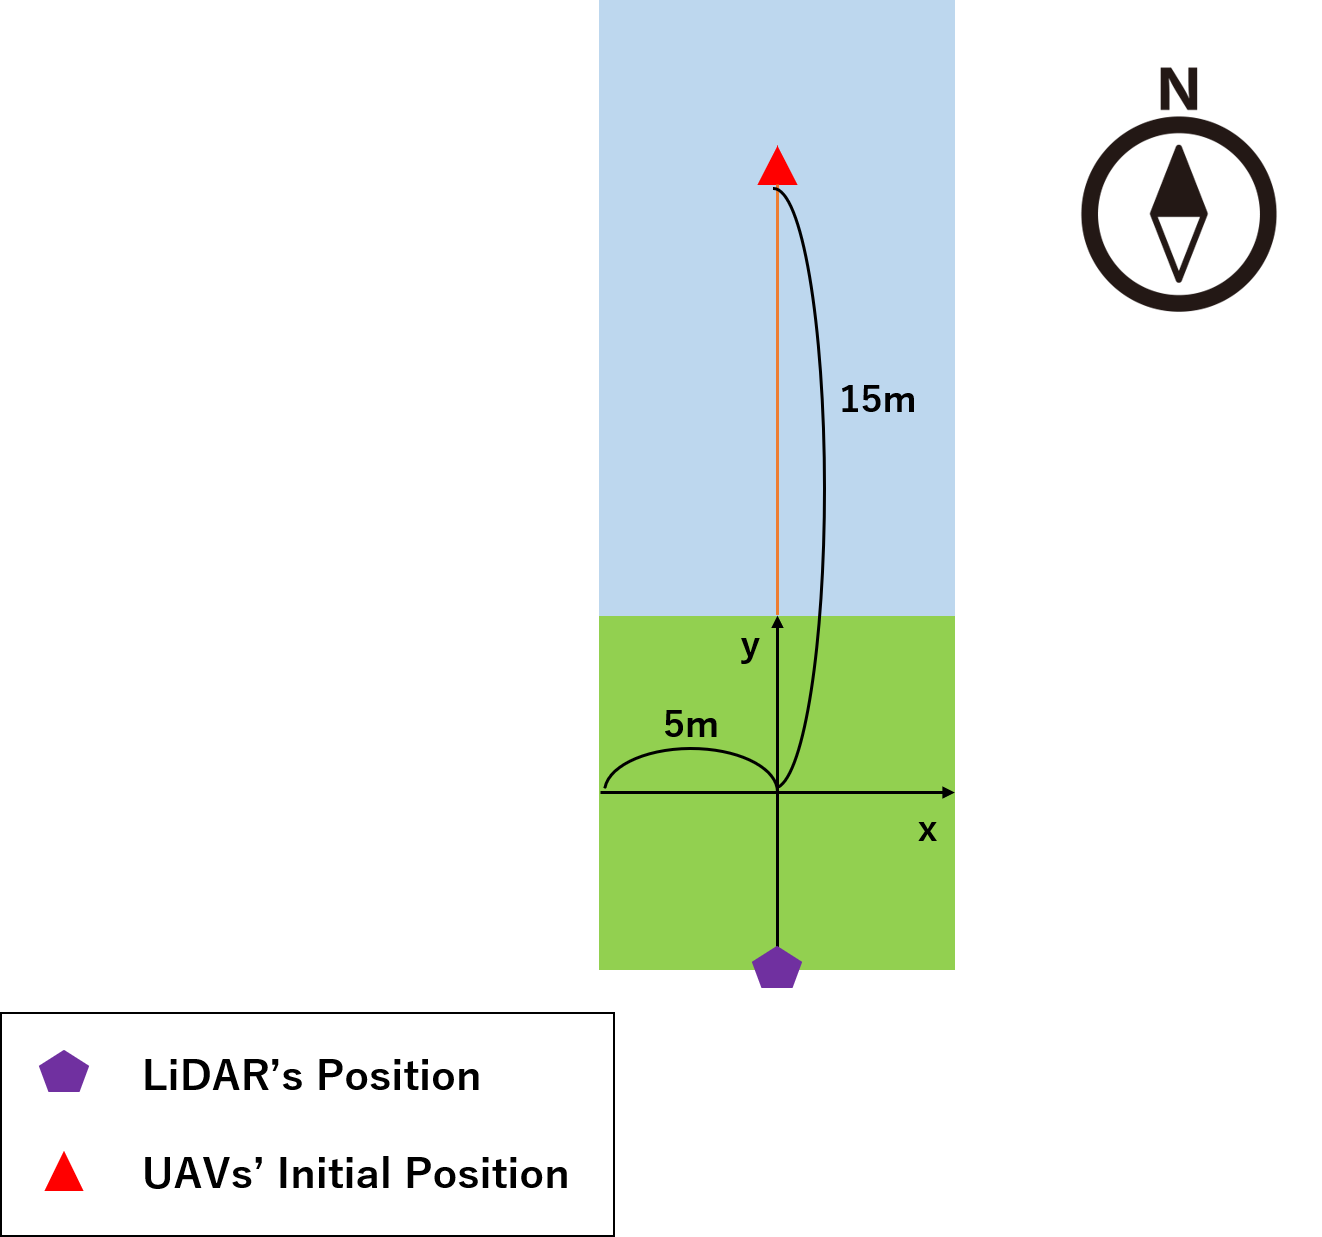
\includegraphics[width=0.6\linewidth, clip]{./figure/chapter5/setting.png}
    \caption{Experiment Environment}
    \label{fig:envi}
\end{figure}

人物の動きを共通なものにするために\cref{fig:pos_person}のような配置を考える.
人物の初期位置は\cref{fig:pos_person}に表す2人の人物の位置とし,図中の矢印に示す通りに移動する.
また図中のバツ印で5秒程度静止する.これを初期位置に戻るまで繰り返し,初期位置戻り5秒程度経過した時点で撮影計画を終了する.
要するに人物の配置が$x$軸上,$y$軸上に並ぶのを交互に繰り返すことになる.

\begin{figure}[h]
    \centering
    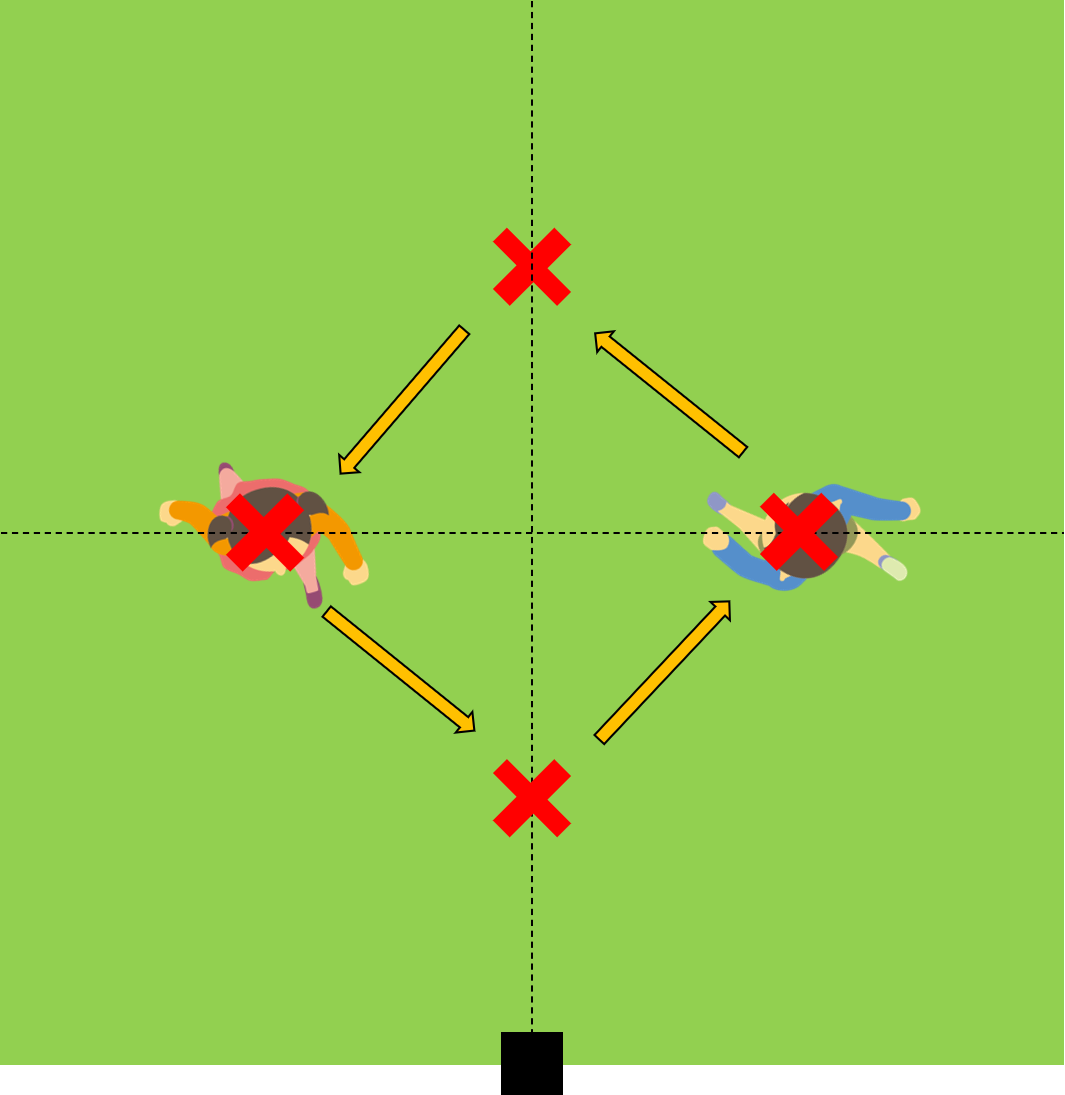
\includegraphics[width=0.5\linewidth, clip]{./figure/chapter5/experience_setting.png}
    \caption{Position of Target Person}
    \label{fig:pos_person}
\end{figure}

\begin{figure}[h]
    \centering
    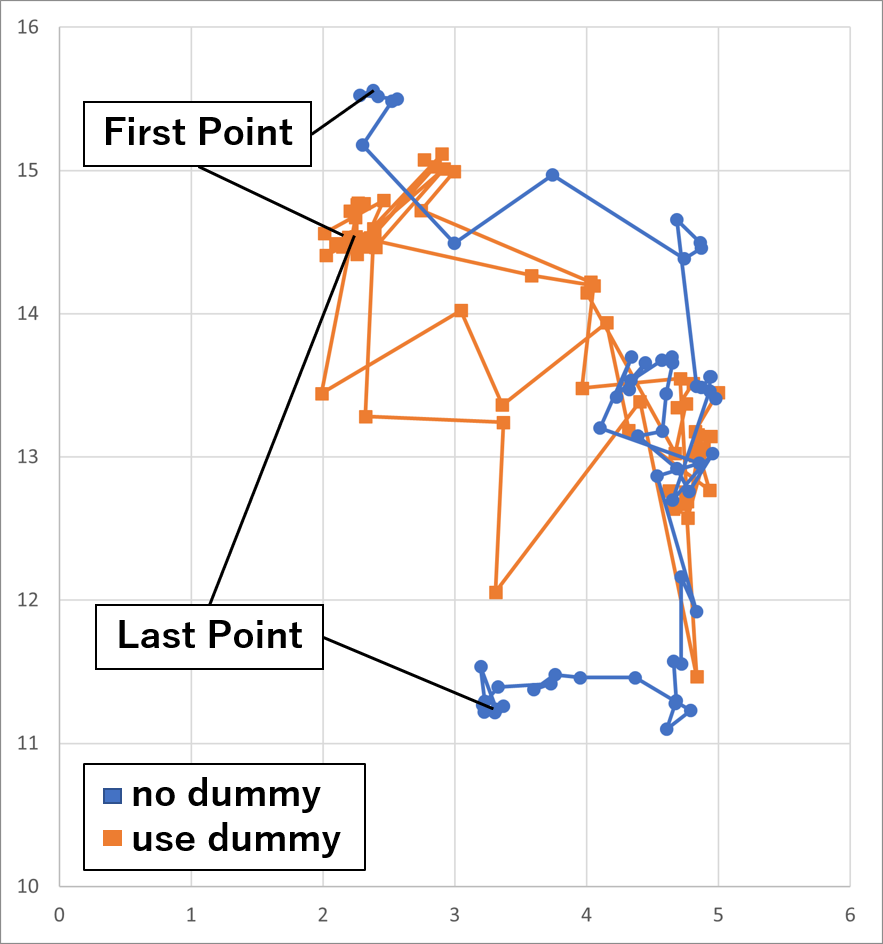
\includegraphics[width=0.5\linewidth, clip]{./figure/chapter5/goal_graph.png}
    \caption{Trajectory of UAV Goal Position}
    \label{fig:pos_person}
\end{figure}

\cref{fig:pos_person}にダミーを配置した場合としない場合に撮影計画を行い,それぞれのUAVの目標位置をグラフ化したものである.
橙色のグラフはダミーを配置した場合のUAVの目標位置であり,青色のグラフはダミーを配置しない場合のUAVの目標位置である.
橙色のグラフは始点から始まり,終点が始点と近い座標に位置している.
これは,撮影人物の初期座標における目標位置位置が始点の位置とほぼ一致していたと推測できる.
それに対して青色のグラフは終点の位置座標が始点の座標の位置より前方に来ている.

3章で説明したダミーの配置方法を使用した場合,ダミーが生成される位置はLiDARから見て人物の後方になる.
そのこと考慮すると,ダミーを配置しない場合のUAVの目標位置よりもダミーを配置した場合の目標位置の方が$y$軸正方向の位置に存在することになる.

ここでグラフの終点付近について考察する.つまり撮影人物が初期位置に戻ってきて撮影計画終了までの時刻付近を考える.
2つの軌跡の終点を比較するとダミーを配置した場合のUAVの目標位置は配置しない場合の目標位置よりの北側に位置しており上記で述べた推測と一致する.このことから3章で述べたオクルージョンエリアを考慮した撮影計画が行えていると考えられる.


\subsection{LiDARを2台用いた人物認識}
次にLiDARを2台設置しての人物認識を行う.
LiDAR1の位置は実験設定で述べた位置に配置し,LiDAR2は南側を向け任意の位置に配置する.
10[m]$times$10[m]の範囲に3人の人物を配置し2台のLiDARでそれぞれ人物認識を行いを3章で述べた方法でそれらの認識データを正常にに統合できているかの考察を行う.また,同一人物とみなす距離$d_{max}$について考察する.

\begin{figure}[h]
    \centering
    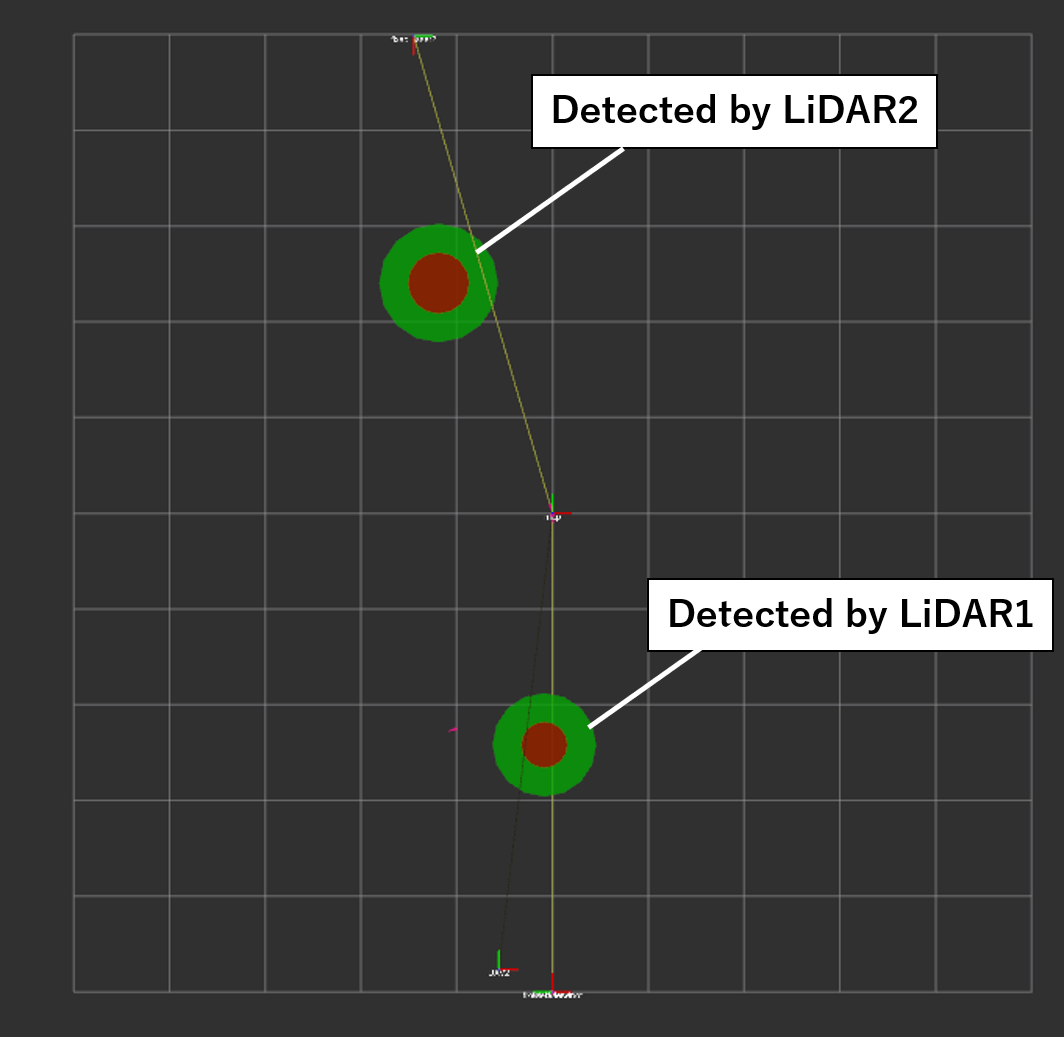
\includegraphics[width=0.5\linewidth, clip]{./figure/chapter5/line.png}
    \caption{Detected Persons in Line by Two LiDARs}
    \label{fig:line}
\end{figure}

始めに2台のLiDARの間に縦に並んだ場合を考える.\cref{fig:line}に各LiDARから検出された人物を示す.
2台のLiDARはそれぞれ各LiDARの前に存在する1人の人物のみを認識しており,縦に並んだ3人の人物のうち中心の人物はどちらのLiDARからも認識されていない.認識された人物をマージする処理を行うと,2人の人物の位置が統合される.


\begin{figure}[h]
    \centering
    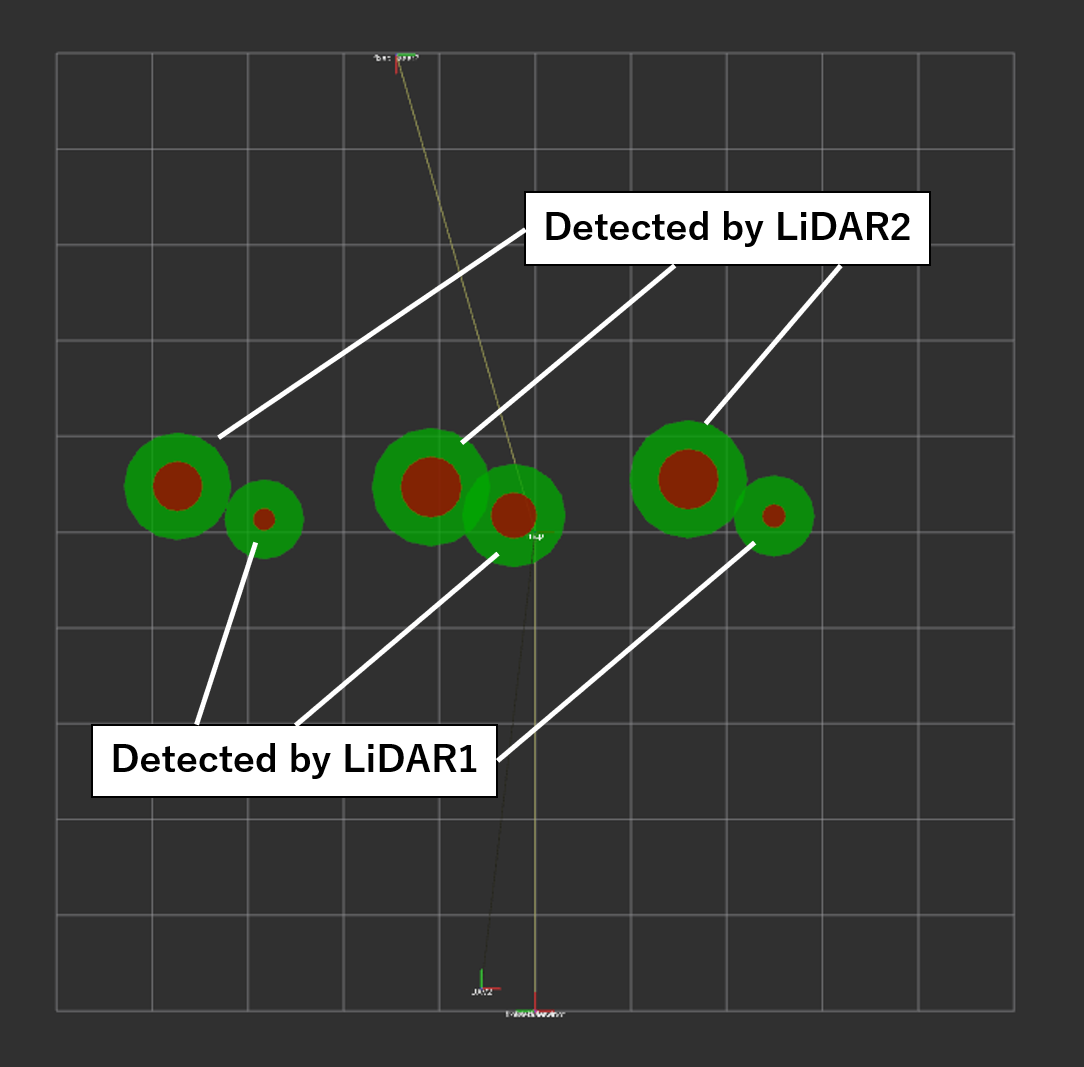
\includegraphics[width=0.5\linewidth, clip]{./figure/chapter5/row.png}
    \caption{Detected Persons in a Row by Two LiDARs}
    \label{fig:row}
\end{figure}

次に2台のLiDARに対して横に並んだ場合を考える.\cref{fig:row}に各LiDARから検出された人物を示す.
2台のLiDARはどちらも3人の人物を認識している.これらの認識された人物にマージ処理を行いに示されている6つの円を3つの円にする必要がある.
各人物を表す2つの円の中心距離を算出し,3章で述べたパラメータ$d_{max}$について考察する.

\begin{table}[h]
  \centering
  \begin{tabular}{|c|c|c|c|c|} \hline
	\multicolumn{2}{|c|}{} & \multicolumn{1}{|c|}{person1} & \multicolumn{1}{|c|}{person2} & \multicolumn{1}{|c|}{person3}\\ \hline \hline
	& $x$ & 2.4269 & -2.8308 &  -0.2124 \\ \cline{2-5}
	LiDAR1 & $y$ &  0.1220 & 0.1694 &  0.1825 \\ \hline
	& $x$ & 1.6752 & -3.7104 & -1.0971 \\ \cline{2-5}
	LiDAR2 & $y$ &  0.5030 & 0.4965 &  0.4432 \\ \hline
 \end{tabular}
\end{table}
\section{本章のまとめ}
本章では2つの実機実験の結果を示し,その結果について考察を行った.

ダミーを配置することにより,配置しない撮影計画と比較してUAVの目標位置が変化することを示した.

次に2台のLiDARでの人物認識について,各LiDARから得られたデータをマージし,そのマージが適切であるかの判断を行った.

次章では,この実験全体に対してのまとめと課題,今後の展望について論述する.


\end{document}
